\section{Structure}
In this section the overall structure of the system will be described using class diagrams.

\subsection{Class Descriptions}
The behaviour of different classes will be described below.

\begin{figure}[tbhp]
	\centering
	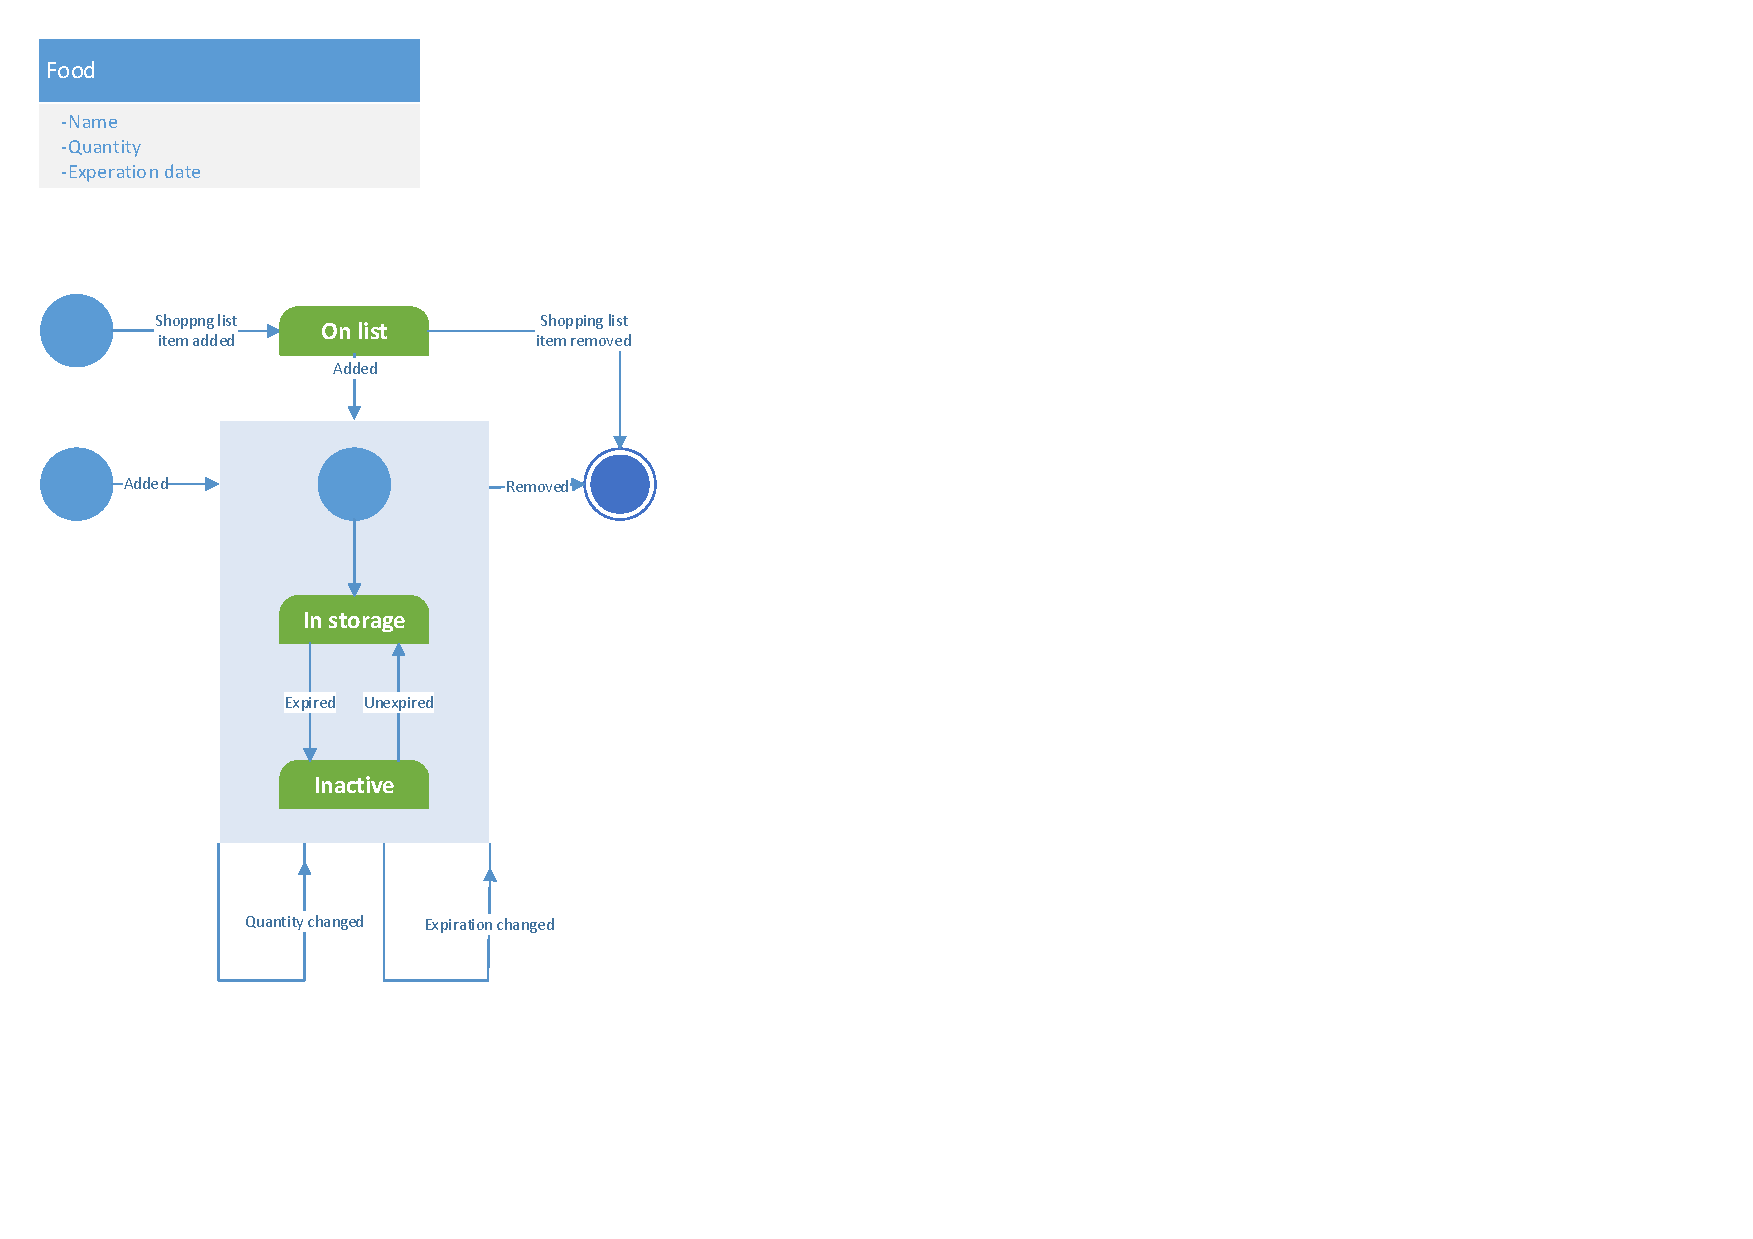
\includegraphics[clip=true, trim=0.5cm 4cm 18.5cm 0.5cm,  ]{Development/ProblemDomain/FoodClass.pdf}
	\caption{Behavior diagram for the food class} \label{FoodClass}
\end{figure}
The \textbf{Food} class contains information about the quantity and expiration date of a food item. The food items can be found in the lists inventory or shopping list.

\begin{figure}[H]
	\centering
	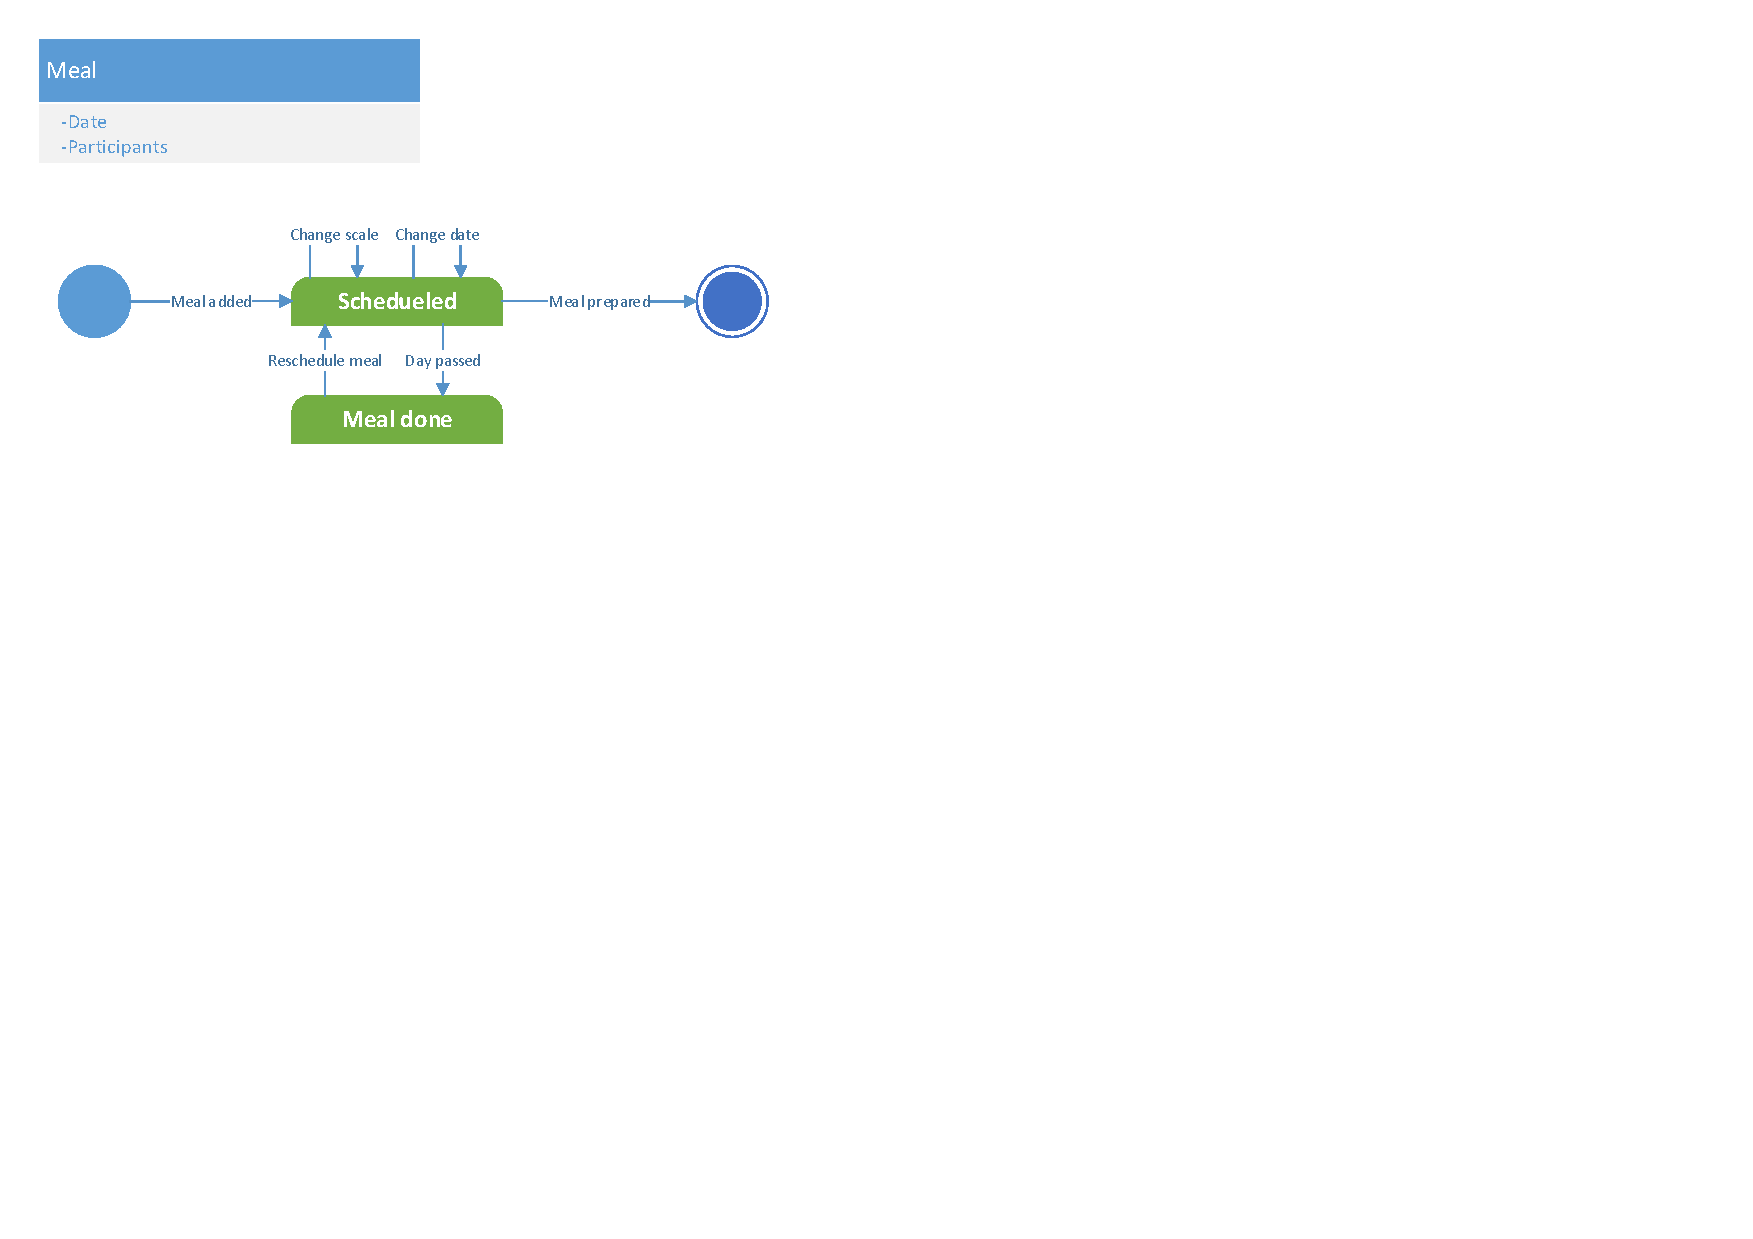
\includegraphics[clip=true, trim=0.5cm 13cm 16.5cm 0.5cm]{Development/ProblemDomain/MealClass.pdf}
	\caption{Class diagram for the meal class} \label{MealClass}
\end{figure}
The \textbf{Meal} class contains information about a meal and when to make it. It consists of recipes.

\begin{figure}[H]
	\centering
	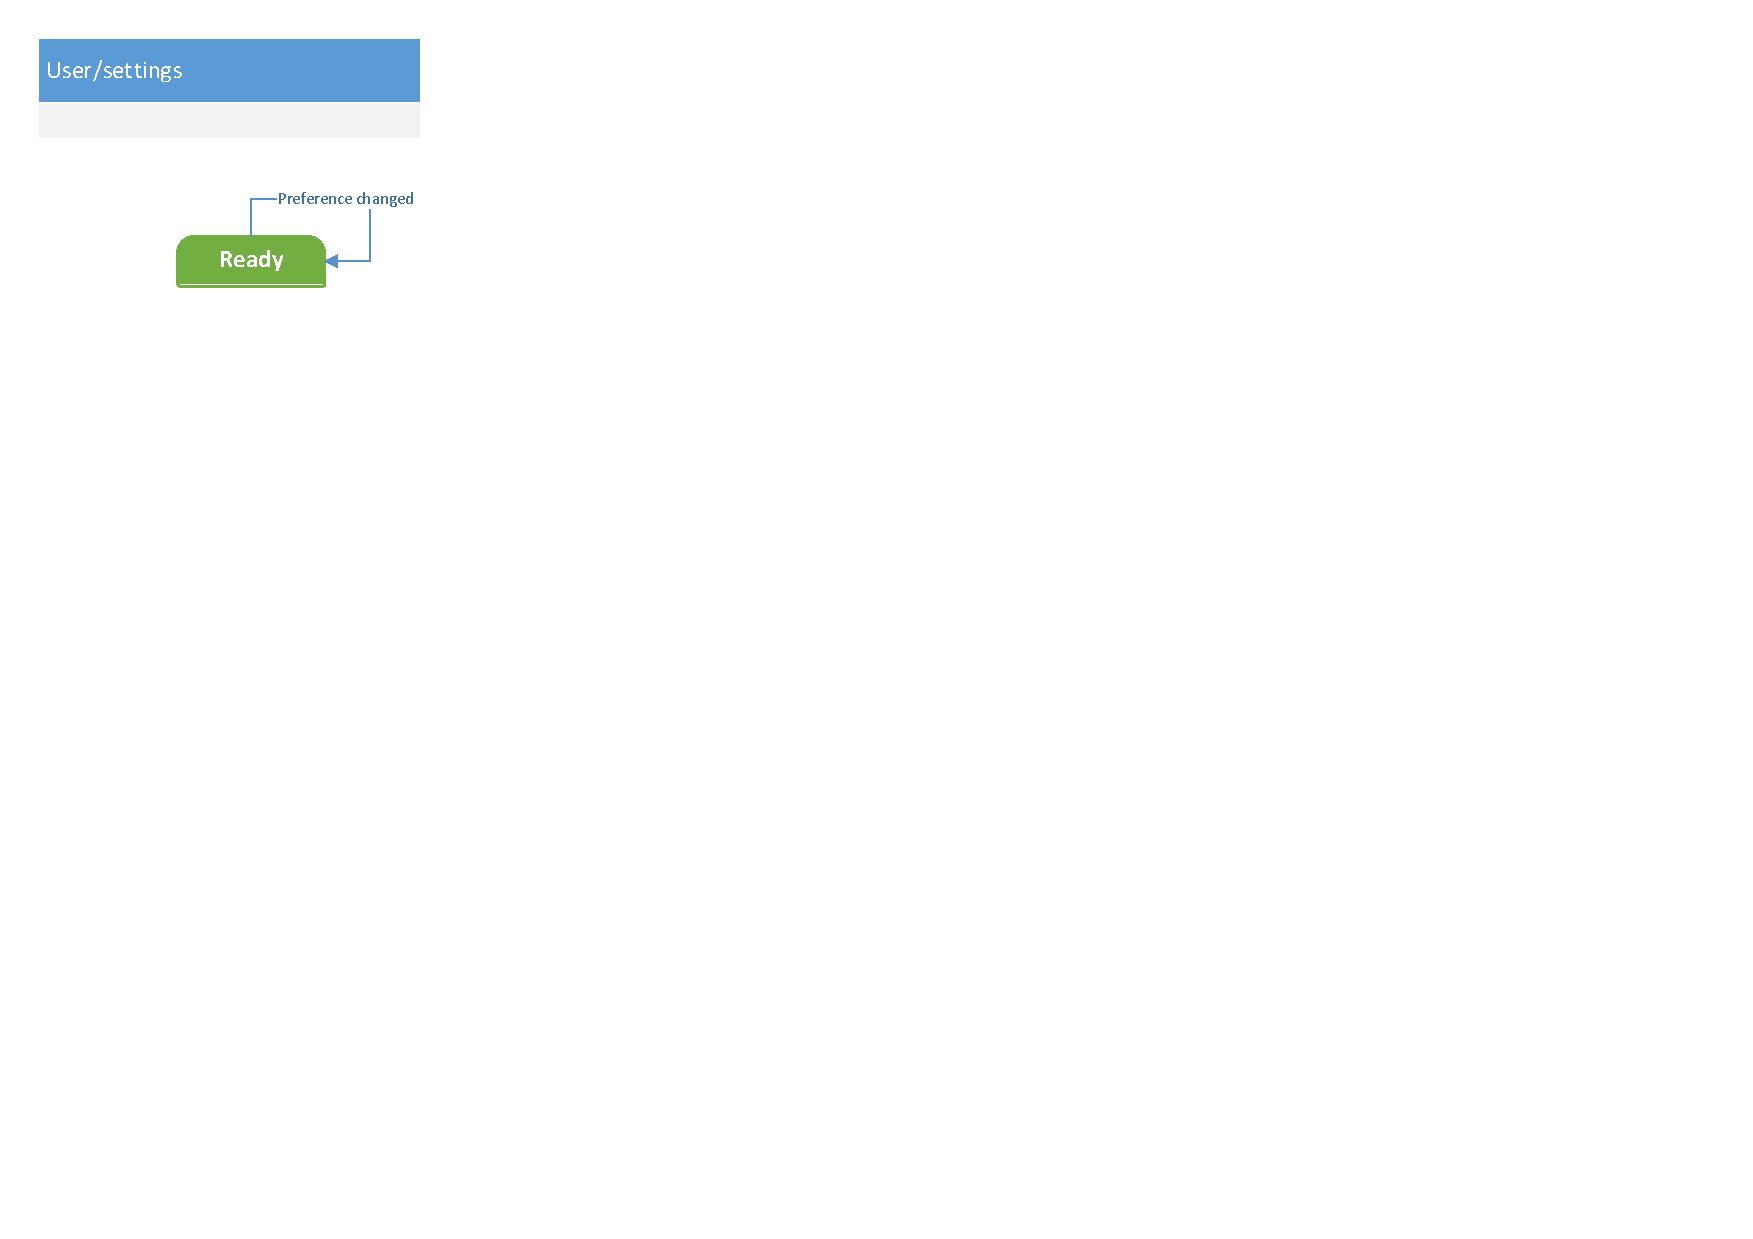
\includegraphics[clip=true, trim=0.5cm 15.5cm 22.5cm 0.5cm]{Development/ProblemDomain/UserSettingsClass.pdf}
	\caption{Class diagram for the user settings class} \label{UserSettingsClass}
\end{figure}
The \textbf{User settings} class contains preferences from the user which the system should take into consideration.

\begin{figure}[H]
	\centering
	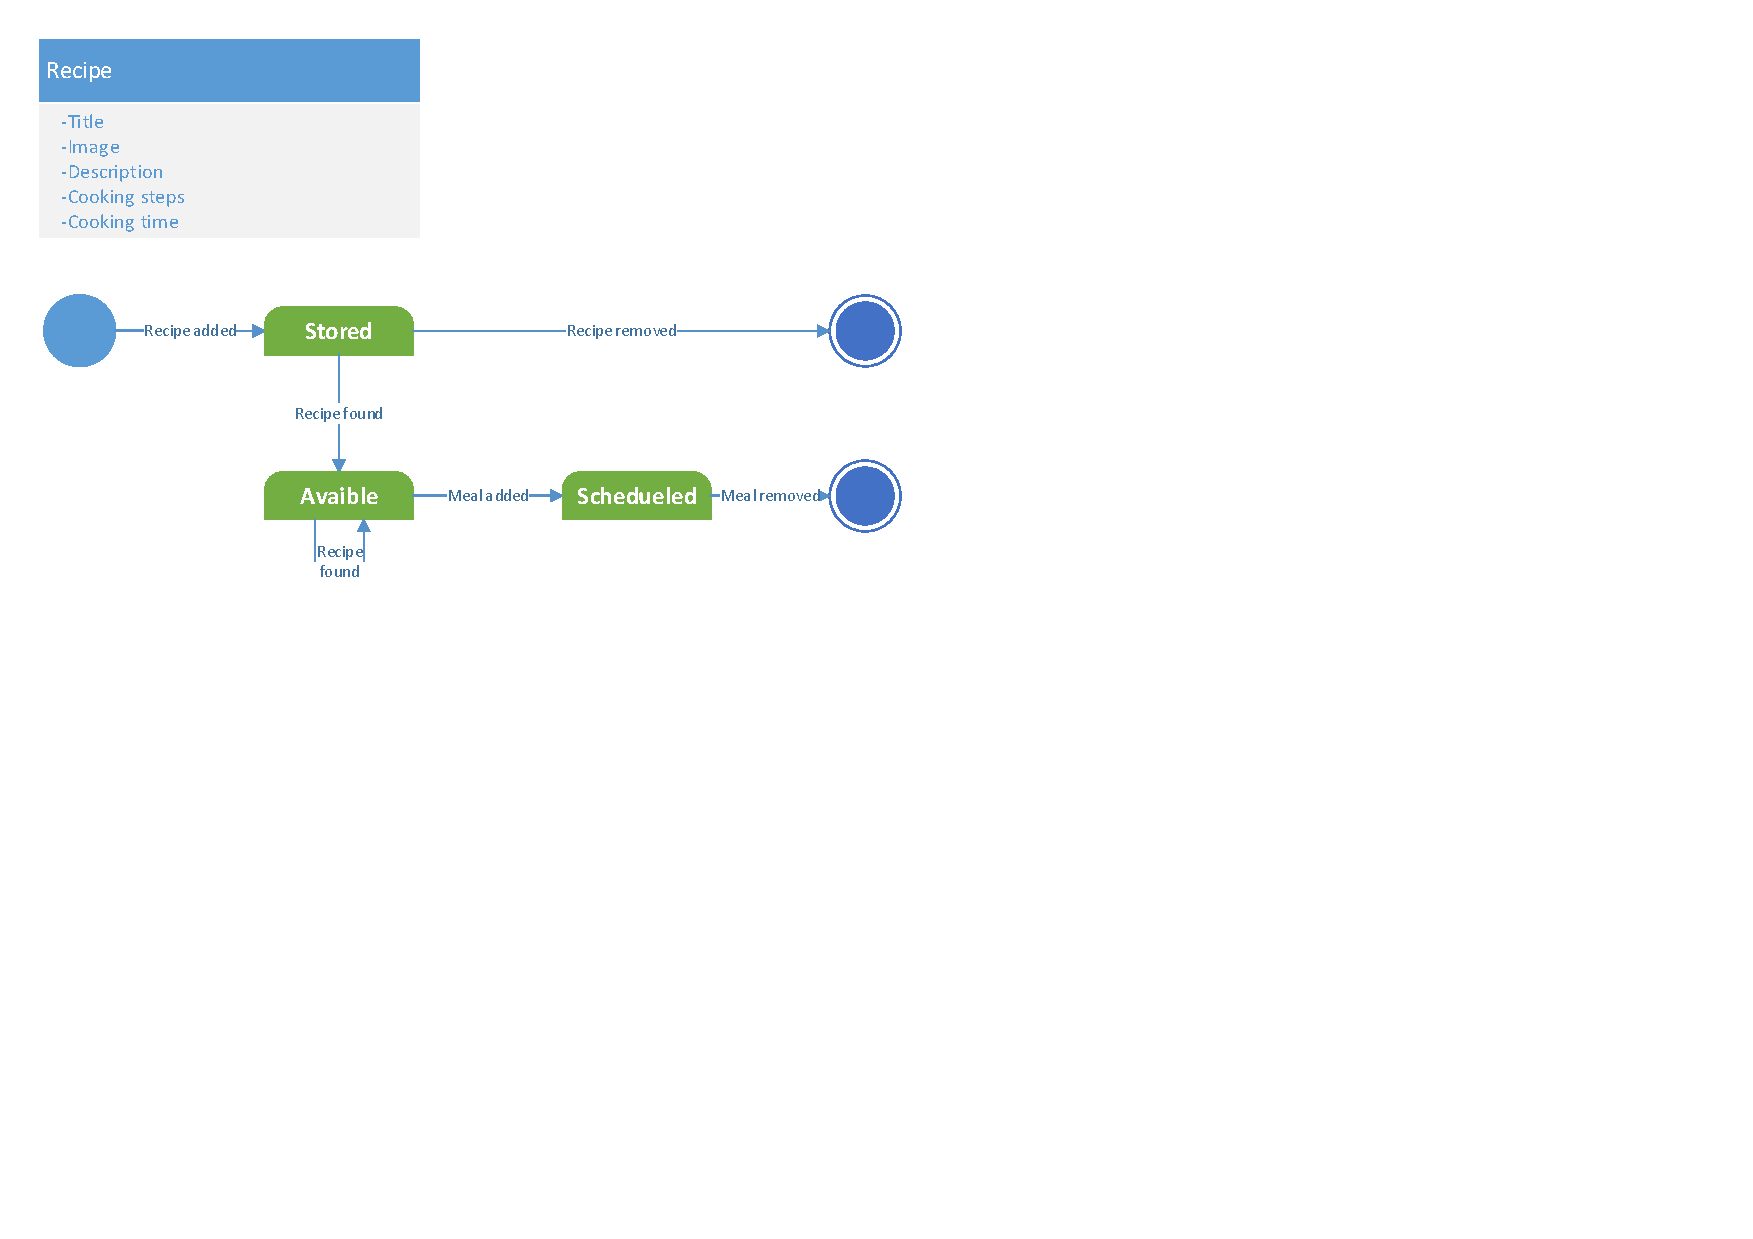
\includegraphics[clip=true, trim=0.5cm 11cm 14cm 0.5cm]{Development/ProblemDomain/RecipeClass.pdf}
	\caption{Class diagram for the recipe class} \label{RecipeClass}
	\end{figure}
\textbf{Recipes} consists of \textbf{Food}. It also contains information on how to prepare the meal from the recipe.

\subsection{Class Diagram}
The class diagram is structured with \textit{Food} as the central class. 
\textit{Shopping List}, \textit{Inventory} and \textit{Foodplan} are lists, containing \textit{Food} or \textit{Meal}.

Food objects can be part of a \textit{Shopping List}, a user \textit{Inventory}, or a \textit{Recipe}, seen as aggregation on \cref{fig:classDiagram}. A \textit{Recipe} contains one to many Food objects, and is part of a \textit{Meal} that in turn is part of a \textit{Foodplan}. A \textit{Meal} contains exactly one recipe, while the \textit{Foodplan} can have any number of planned \textit{Meals}.

\begin{figure}[H]
	\centering
	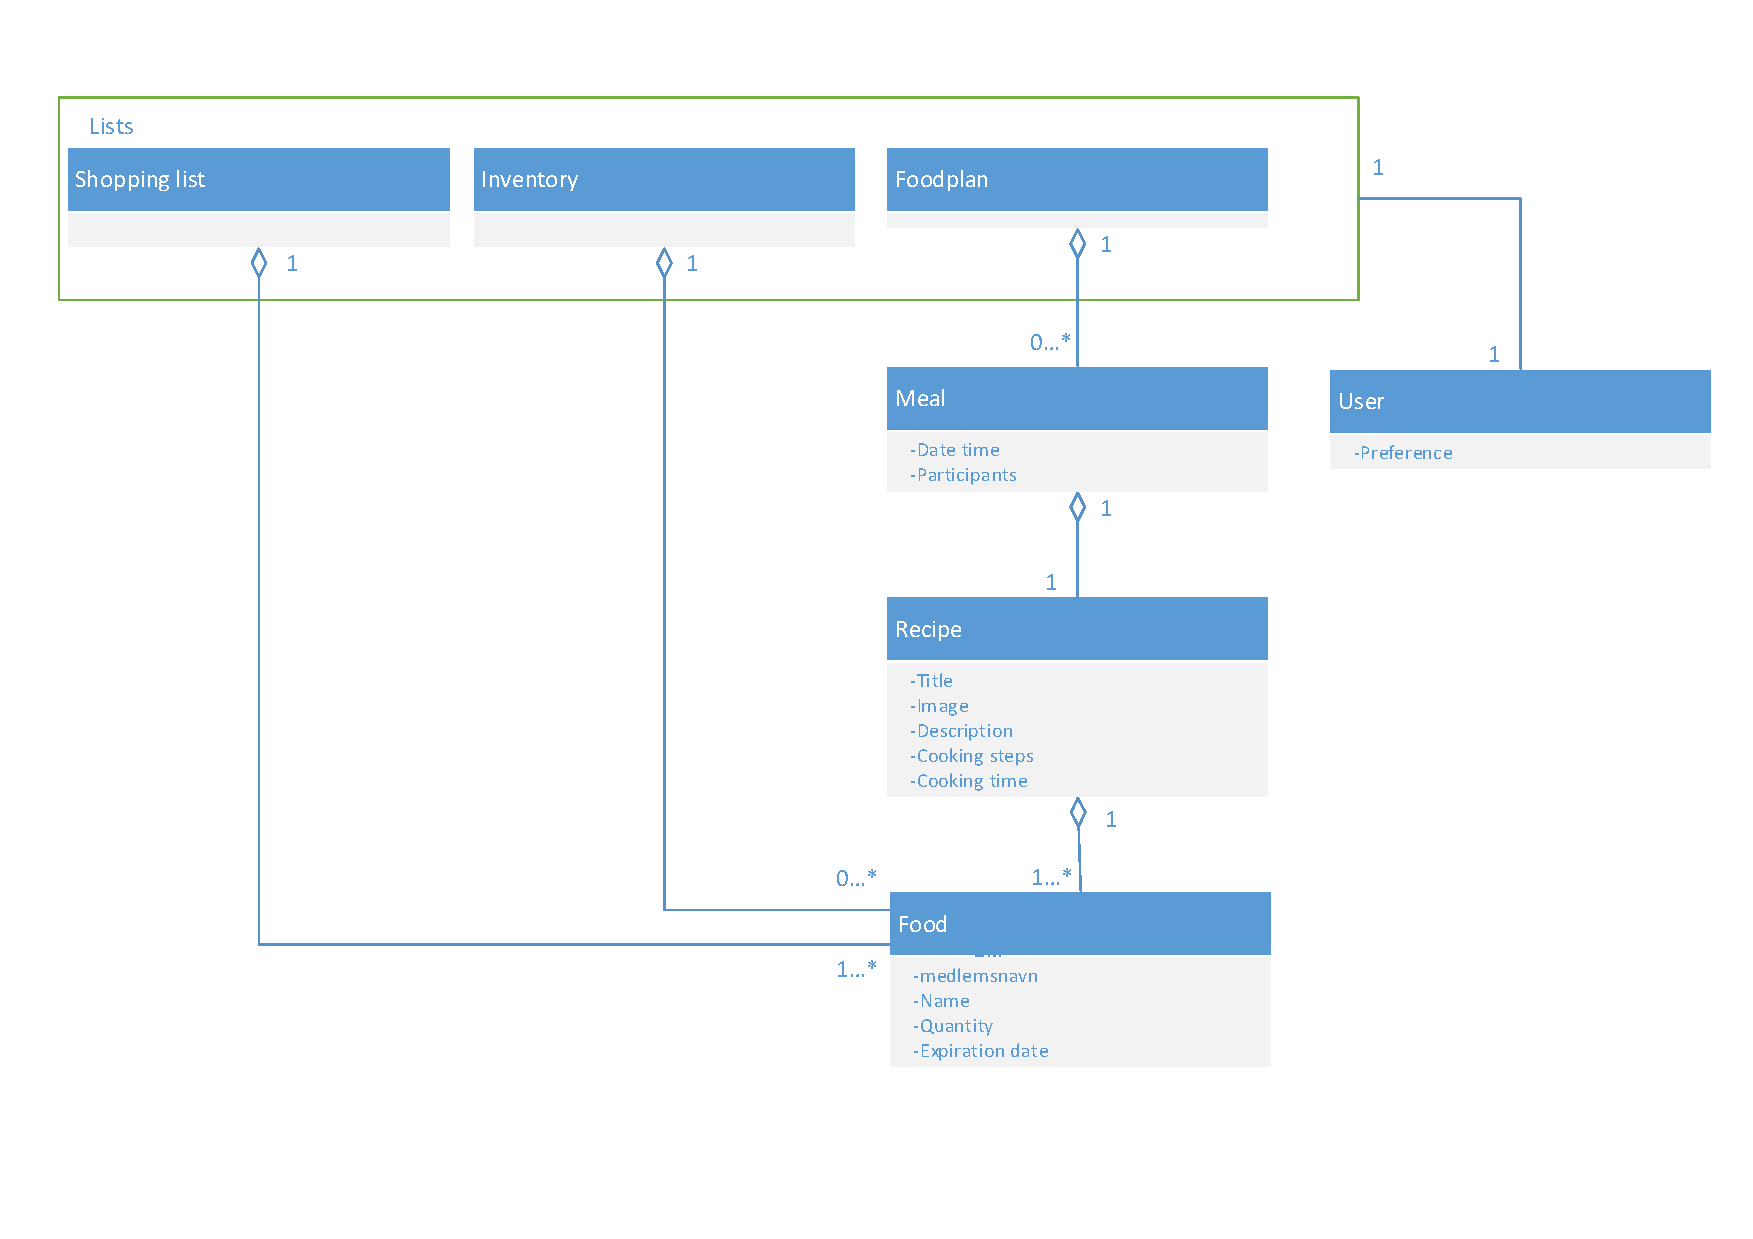
\includegraphics[clip=true, width=1\textwidth, trim=1cm 3cm 4cm 0]{Development/Klasseting}
	\caption{Relation between classes.}
	\label{fig:classDiagram}
\end{figure}